\documentclass[titlepage, a4paper,10pt]{article}
\usepackage{appendix}
\usepackage[margin=2.5cm, nohead]{geometry}
\usepackage{graphicx}
\usepackage[all]{xy}
\usepackage{pdfpages}
\usepackage{hyperref}
\usepackage{verbatim}
\usepackage{color} % for todo
\usepackage{subfig}
\usepackage{fancyhdr}

\renewcommand{\headrulewidth}{.2pt}
\renewcommand{\footrulewidth}{0.2pt}

\setlength{\headsep}{1.0cm}
\setlength{\voffset}{-1cm}

\pagestyle{fancy}
\rfoot{\thepage}
\cfoot{}
\lfoot{\footnotesize AP2DX}
%\addtolength{\footskip}{5pt}

\newcommand{\todo}[1]{\colorbox{red}{\color{white}#1}}

\begin{document}


\newcommand{\HRule}{\rule{\linewidth}{0.5mm}}

\begin{titlepage}
\begin{center}

\includegraphics[width=1\textwidth]{uva}\\[0.5cm]

\HRule \\[0.4cm]
{ \huge \bfseries \LARGE Awesomizing the P2DX }\\[0.1cm]
\HRule \\[0.4cm]

\textsc{\LARGE AP2DX}\\[0.5cm]
%\textsc{\small AP2DX}\\[1cm]

%\begin{tabular*}{0.95\textwidth}{@{\extracolsep{\fill}} l c r}
%Jeroen \textsc{Rooijmans}	& Maarten \textsc{Inja}     & Maarten \textsc{de Waard} \\
%\textsc{5887410}                &\textsc{5872464}           &\textsc{5894883}\\
%\end{tabular*}

\begin{tabular*}{0.95\textwidth}{@{\extracolsep{\fill}}c c c c}
Wadie Assal & Jasper Timmer & Maarten de Waard & Maarten Inja \\
6398693 & 5995140 & 5894883 & 5872464 
\end{tabular*} \\
\vfill \large \today
\end{center}
\end{titlepage}


%\thispagestyle{empty}
\tableofcontents 
\newpage
%added a newpage after every chapter so it looks more like a report then a article. Wadie Assal

\section{Preface}
As a part of the course Software Engineering and Distributed Applications, of
the University of Amsterdam, we are asked to program a distributed application
for a virtual robot. The team consists of students with different profiles:
three are from Artificial Intelligence, one from Computer Science and ICT at the
Amsterdam University of Applied Sciences and one from the pre-master Software
Engineering. This melange is both a chance to create something good from
different viewpoints as well as a point of attention, because none of us has
followed the bachelor Computer Science at the University of Amsterdam. 

\subsection{Chairmans ``Who has written what?''}
In the Blackboard document ``Huishoudelijk Reglement'' is written that the chairman should declare who has written which
part of this report. This is not an accurate representation of the division of labor, but here it is:
\begin{itemize}
    \item Introduction. Japser Timmer
    \item Architecture and results, everyone
    \item Building and testing, Jasper Timmer
    \item Discussion, Maarten de Waard and Maarten Inja
    \item UML Diagram, Waddie Assal
\end{itemize}
\newpage

\section{Introduction}
For the client a robot controller that can autonomously map an area had to be build. This was attempted in less than four weeks. After two and three weeks there were milestones to show the client the progress.

\subsection{USARSim}
As simulator USARSim is used. USARSim (Unified System for Automation and Robot Simulation) is an application to simulate the real robot arena's of the IEEE, based on the Unreal engine. The robot should be able to navigate through the 'Yellow Arena'. This is a map with a few static obstacles.

\subsection{Goals}
With the client is agreed to build the following features in the robot-controller:
\begin{itemize}
\item Loosely coupled modules based on network communication
\item Robot should be safe, i.e. stop for obstacles
\item Robot should be able to drive autonomously through the environment
\item Robot should be able to create a map of the environment
\end{itemize}

\subsubsection{Milestones}
This section will describe the milestones, and what deliverables we will provide. 

\subsection*{Milestone 0}
This will describe what we will have done by the 10th of June. These are the
deliverables:
\begin{description}
\vspace{0cm}
\item[Working environment:] We will set up a Git
repository\footnote{https://github.com/Y3PP3R/AP2DX} and a testing environment
(using jUnit).
\item[Base class:] We will make an abstract base class, on which we can base
all our Java classes. This will contain all the standard methods, e.g. TCP/IP
protocols.
\end{description}

\subsection*{Milestone 1}
This will describe which deliverables we will have done by the 
\begin{description}
\item[Drive:] We want the program to be able to direct
the robot through the environment. We will not yet focus on the ability to
follow lines or walls.
\item[Avoid collision:] The robot should be able to avoid collision with objects
and walls. It will stop, turn a random corner, and drive on. This way it will
cover most of the area without colliding.
\end{description}

Classes needed to be implemented for these goals:
\begin{itemize}
\item Co\"ordinator
\item Sensor
\item Reflexes
\item Motor
\end{itemize}

\subsection*{Milestone 2}
A list of deliverables:
\begin{description}
\item[Avoid obstacles:] The robot will be able to avoid the obstacles that
cross his path, in stead of stopping and turning a random corner.
\item[Navigate:] The robot will be able to navigate through the room.
\end{description}

What we will implement for this:
\begin{description}
\item[Mapper:] A class that creates a map of the room out of the sensor
data. In the time of milestone 2 it does not have to be able to create an entire
map and be very accurate, but it will be able to make some implementation.
\item[Improved Sensor:] The sensor class will be improved to be able to make
an accurate map.
\item[Improved Reflexes:] The reflex class needs to be able to use some
sensor data to be able to avoid objects appropriately. 
\end{description}


\subsection*{Demonstration}
Before the demonstration we will be able to do the following things:
\begin{description}
\item[Planner:] We will have a planner class that can specify directions
based on the current map position and what part of the map we have not yet
discovered.
\item[Improved Mapper:] The mapper will now be able to make an accurate map
and find our location on it, while taking the errors in sensor data into account.
\item[Tests:] Although we test all the time, we want to have tested
everything good before the end.
\item[Report:] We will work on a report, describing our progress, problems
and (test)results.
\item[Documentation:] We will work on a proper documentation of our code,
which is also finished before the end.
\end{description}

The classes we will need to implement or improve for this are:
\begin{itemize}
\item Mapper
\item Planner
\item All test classes
\end{itemize}

\subsection{Structure of this document}
This document is written for the client as reference about the delivered software. It contains information about the architecture of the program (all the components) and design desicions. Also the development and test process is described. The last part is about what is actually deliverd and what can be improved. In the appendices there is more indepth technical information.

\newpage

\section{Architecture \& Results}
\subsection{Introduction}
AP2DX is written completely in the Java programming language. 
This was chosen as it is advertised to be reliable and fast by the company Flowtraders, and it is platform independent. This is important for AP2DX, because it should be a safe robot controller, that stops in time and does not harm anyone on it's path. The architecture of AP2DX is based on Object Oriented Programming (OOP).
To not repeat the same code again and again for every module, a baseclass was constructed. 
This class could do things as: read a config file, write to a logfile, accept incoming connections, start outgoing connections based on the config file, handle incoming messages and send responses.
The baseclass was designed to be flexible for the needs of every module. Also, the program is heavily multithreaded, to open and check connections and to do the business logic and send messages. As for the messages: a base message class was build, to facilitate the communication between USARSim and AP2DX, and between modules of AP2DX. As standard for config file and communication, JSON (Javascript Object Notation) was used. 

\subsection{USARSim}
\begin{figure}[b]
  \centering
  \subfloat[The original P2DX]{\label{fig:p2dxReal}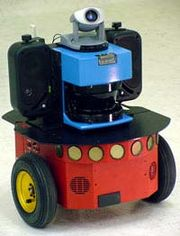
\includegraphics[height=0.2\textheight]{p2dxReal}}                
  \subfloat[The P2DX in USARSim]{\label{fig:p2dxUsar}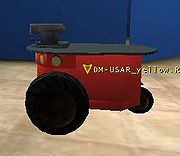
\includegraphics[height=0.2\textheight]{p2dxUsar}}
  \caption{The P2DX we worked with}
  \label{fig:p2dx}
\end{figure}
The simulator exists of a virtual enviroment where different maps and different
robots can be loaded. These robots have different sizes and different features.
As example of features of a robot, there are different kinds of sensors and
different kinds of wheels. For AP2DX, the robot P2DX (See figure \ref{fig:p2dx}) was used. This robot is a three-wheel, rear swivel wheel robot. The two frontwheels can be controlled independently of eachother, so it is possible to turn almost in place. As sensors are available on the P2DX:
\begin{itemize}
\item 8 Sonar distance sensors
\item Laser distance sensor
\item Odometry sensor
\item Inertial Navigation Sensor
\item Camera
\end{itemize}
For the purpose of AP2DX only sonar, laser and INS sensors are used.
\subsection{Coordinator}
The first module a message on a journey from the USARSim to AP2DX meets, is the AP2DX Coordinator. The Coordinator is programmed to spawn the robot and translate and relay traffic between the simulator and the AP2DX System. That is all it really does. It has a connection with the Sensor module to relay the incoming sensor data and the Motor module to receive commands for the simulator.

\subsection{Sensor}
\begin{figure}
\centering
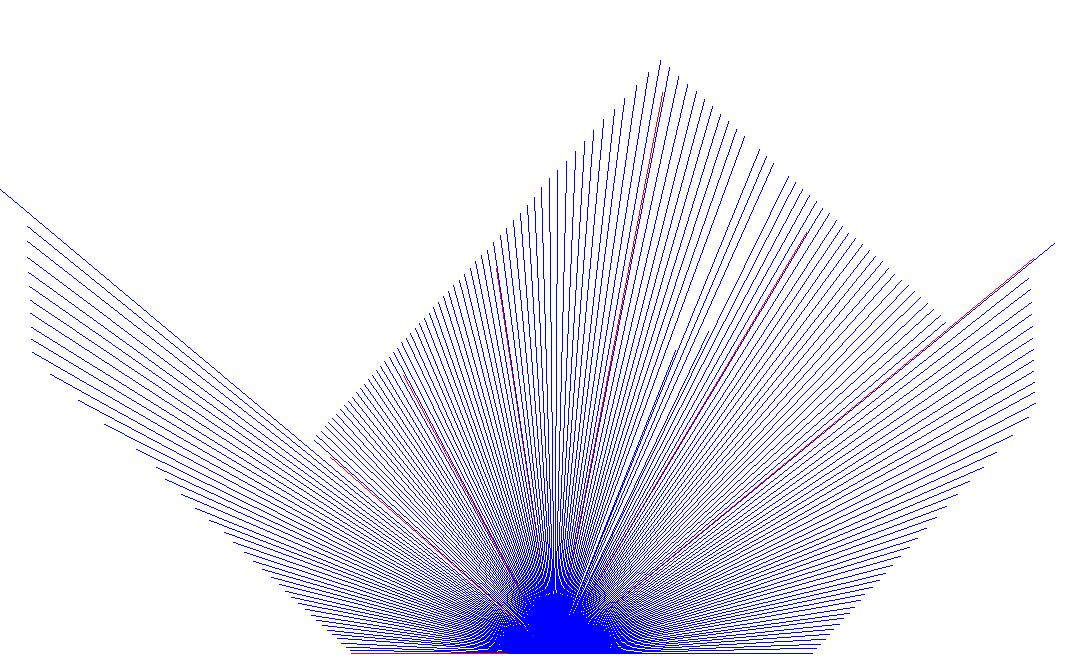
\includegraphics[width=.7\textwidth]{Sensor.jpg}
\caption{The data from the laser range scanner and the sonar, as represented by
our program. Red represents sonar data, blue represents laser data.}
\label{fig:sonarLaserData}
\end{figure}

The sensor module has two tasks. The first task is forwarding different kind of 
sensor messages to the mapper module and the reflex module. The second task is to
display the sonar and range scanner (laser) sensor data graphically. This allows 
to see if the data is correctly parsed by the coordinator module and received by 
this module with one quick glance. Furthermore it can be used for other debug 
purposes, such as checking correct reflex behavior. See figure \ref{fig:sonarLaserData}
for an example of displayed sensor data. 




\subsection{Mapper}
The task of the mapper module is to create a map of the environment and to find the position of
the robot in this map. This will allow the planner module to plan paths and other behaviour, that is:
if it is done correctly! 

Luckily, simultaneously localizing and mapping (SLAM) 
%creating a map and simultaneously localizing a robot 
is a commonly encountered problem and 
many research has been conducted to optimize algorithms. The mapper module uses the \emph{DP-SLAM}
\footnote{\url{http://www.cs.duke.edu/~parr/dpslam/}} implementation in the C programming language.
Starting the DP-SLAM program (which was slightly modified for compatibility with the Java module)
is done with a system call, after which two threads are started. One to write the correct sensor 
data to the input stream of the program, and one to read the output stream of the program. The 
output stream contains information about for example the location of the robot, whether or not
something went wrong or when a new map has been dumped to file.

Unfortunately, the mapper module is not multi platform as the DP-SLAM program uses Linux libraries. 
If this module is run in a non Windows system no map can be created, but sensor important data will
still be forwarded to the planner module. 




\subsection{Planner}
The planner controls the robot movement. It uses sonar, odometry and INS data to determine the next action to take. The Planner has three behaviors: drive and turn away from obstacle, check out gaps in the wall and get free from a stuck position.

\subsubsection{Behavior: Drive}
The robot starts driving when the first sonar data is received. The outer two sonar sensors are ignored, but the inner six are used to determine if the robot is approaching an obstacle and the distance is under a certain threshold constant. Then the Reflex module kicks in and sends a stopmessage to the robot and the Planner. The Planner then checks if the sonars on the left or on the right have the most far view and turns in that direction, until the robot has no obstacle in front of it anymore. This is calculated as follows: If the first of the eight sensors has number 1, and the next number 2, etc. the sensors 3 and 6 are in an angle of 60 degrees. This means it is an equilateral triangle if sensors 3 and 6 can see the same distance, and that means, if the sonars 3 and 6 can see at least as far as the robot is wide, it will be possible to drive forward. A small margin is added to the width to be sure the robot does not get stuck.

\subsubsection{Behavior: Check hole}
When the sonars 1 or 8, that are perpendicular on the robot's path see a difference between two sonardata sets, that is larger then a certain threshold, say 1 meter, the robot gets curious and wants to to know if there is a hole beside it that it can drive through. It turns 90 degrees in the direction of the hole, scans if the hole is wide enough and drives forward if it is. Is it too small, then it turns back and continues it's original path.

\subsubsection{Behavior: Get free}
Every time INS data is processed, the planner checks how much the robot has moved since the last INS data. If this is under a certain threshold, the robot increments a counter. If the robot did not move enough after a certain amount of INS data, it goes into 'stuck' mode: stop doing things, drive backwards for a small distance, turn 90 degrees left or right at random and start scanning for a new path.

\subsection{Reflex}
The Reflex does only two things. Relay motor messages from the planner to the motor, and stop those messages if there is something in front of the robot, so it has to stop. If it has to stop the robot, it sends a stop message to both the motor and the planner and discards all the movement messages it receives from the planner until the planner sends an acknowledge message.

\subsection{Motor}
The motor module translates motor messages into motor messages. If it gets forward, 10, it translates to leftwheel 10, rightwheel 10. It does not yet create usarsim message, but it sends this message to the Coordinator and there it is translated and send to the simulator.

\subsection{Communication}
% Misschien moeten hier wat subsecties bij, kan bovendien wel netter taalkgebruik worden
There are two seperate protocols in use in AP2DX. The first protocol is the Gamebot protocol 
used by Unreal Tournament to communicate with the simulation. The coordinator module is the 
only module that uses these messages. First the coordinator module sends a ``spawn'' message 
to create the robot in the simulator. Then it continues to read messages (often containing 
sensor data) send by the simulator and to send messages (containing ``drive'' commands) to
the simulator. 

The second protocol is the AP2DX message protocol. These are JSON strings that \emph{always}
contains a source module ID, a destination module ID and lastly a type, indicating what kind
of message this it is. Other data in these messages might vary. For example; a sonar sensor
message has the sonar data in it. A drive message only stores the information on how to drive
in the string. 
This protocol is used to communicate between all the modules in 
AP2DX.  The coordinator module is responsible for translating messages using a kind of
protocol to a message using the other kind of protocol.

Using two protocols meant that a lot of things had to be done twice, but also that a module 
could deal with both protocols. Thefore the 
base class deals with instances
of our abstract ``Message'' class and has an interface ``IMessageParser''. Final modules \emph{knows}
what kind of protocol a connection uses and can set up the right message parsers (``AP2DXMessageParser'' 
or ``USARSimMessageParser'') and thuss, deal correctly with the incoming messages. 

Different kind of messages need to be dealt with as well. The source and destination module ID take care
of getting the message to the right module. The type is used to identify a message. Once a message
has been identified as, for example a range scanner sensor message (type: AP2DX\_SENSOR\_RANGESCANNER), 
it becomes a ``specialized message''. 
A specialized message parses the variables in the string and sets them in variables in the message. Now,
simple setters and getters can be used to modify and read all the different 

The hierarchy of our messages can be seen below: 
TODO: picture; Message to AP2DXMessage and USARSimMessage. AP2DXMessage to SpecializedMessage. SpecializedMessage
to all the sensor messages and motor messages and drive messages. USARSimMessage to Jaspers messages. 



\newpage

\section{Building and Testing}
In this section, we will explain the way we tested our program, and automated our build process. Developing and debugging involve a lot of the same actions. To make the development process less repetitive, tedious and time consuming, some manhours were spent on setting up a good working environment. A git repository was setup at github.com. To develop better code, there was the idea to start with building unittests before actual code. More on unittests later. To automate the compiling, testing, building of Javadoc and creating Java executables (.jar files), an Ant buildscript was created. Next a continuous integration server was set up.

\subsection{Git}
Git is a distributed version control system, not like Subversion, but like Mercurial. Git allows the developers to work on the same file together and merge the changes. Every commit is only made local and can be reversed. A project was started at http://www.github.com that free Git versioncontrol for opensource projects. It also offers development statistics, wiki and issue management, but those features were not used.

\subsection{Ant}
Java was chosen for AP2DX, and Java has to be compiled before it can be run. Also, the build directory has to be cleaned, unittests have to be compiled and run, Javadoc has to be published and executables containing the compiled classes had to be generated. This whole process can be automated with an Makefile-like tool, called Ant. An Ant Makefile is called build.xml. When in a terminal in the directory containing build.xml, all the developer has to do it type 'ant' and the process is run. Because developers don't want to wait on javadoc and testing to be completed every time they need to compile and debug, a second build target was created that only did the compiling and generating of jar files, and this could be run with 'ant debug'. Jenkins did run the full buildscript.

\subsection{Jenkins}
To put everything together and test if it still works, a continuous integration server can be used. Jenkins was choosen for good reviews, and personal experience. What it does, is get every whole hour a clone of the Git repository, execute the Ant script, and publish the testresults. Jenkins is a java program and was run from a student home directory on deze.science.uva.nl, during development hours.

\subsection{Testing}
The original idea for the development of AP2DX was Testdriven development. This involves writing unittests before the actual code using jUnit testing framework. The idea of a unittest is to test the smallest possible unit of code, this is a class method or constructor. A good unittest is independent of other classes. If one class fails, the test for the class that is dependent on the failing class should not fail, because this class may be written correctly. It is possible to make unittests independent on other classes, with class mockups (using the jMockit framework), that are something like dummy objects, that do exactly what you want them to, but this is subject for an other paper.

It is not only important to write tests that test all methods and all possible input and output values, but another measurement instrument for the quality of the tests is line coverage. it is almost never possible to get 100\% line coverage, but about 80\% line coverage should be well tested code, if all possible input and output values are covered. There are more metrics then line coverage like package coverage or conditional coverage, but in this project the focus was on line coverage. This is expressed in the number of lines with executable code which are reached by the tests, as visible in figure \ref{fig:hits}.

\begin{figure}[h]
  \caption{Hits per line}
  \centering
    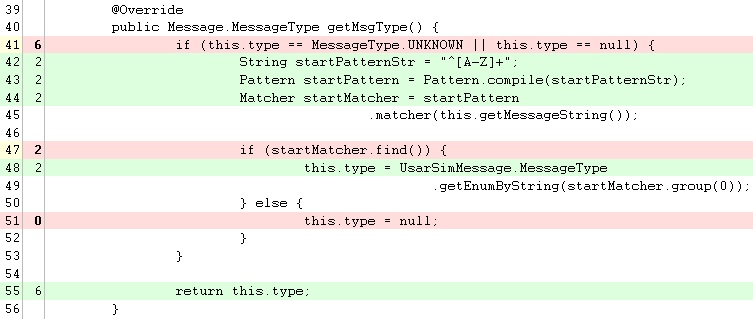
\includegraphics[width=0.5\textwidth]{hits}
  \label{fig:hits}
\end{figure}

Writing of tests was harder than planned and took to much time, so it was decided to stop that and start working on the robot controller. Testing requires a specific mindset and understanding of the process, and because of the socket communications testing was not that simple. it is possible to mock a socket but mocking is difficult also, and it is possible to start a listing socket and let the class under test connect to it and then send it a message, but this requires extra threads which is not very handy for unittests.

\subsubsection{Testreport}
In the final product the quality guideline of 80\% line testcoverage was not met. This was because of a couple of before mentioned reasons. The final testresults are very good: only 30\% line coverage and 10 failing tests on a total of 58 tests (figure \ref{fig:coverage} and \ref{fig:tests}). The figures show the results of the last successful build attempt with no failing tests and the last nine build attempts, where the last one (236) is the one that is actually delivered.

\begin{figure}[h]
  \caption{Test coverage}
  \centering
    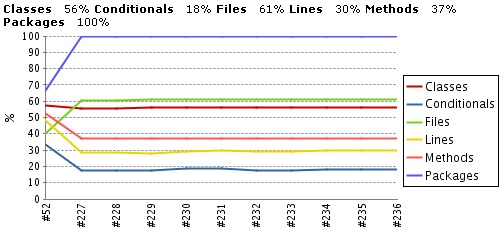
\includegraphics[width=0.5\textwidth]{coverage_graph}
  \label{fig:coverage}
\end{figure}

\begin{figure}[h]
  \caption{Test results}
  \centering
    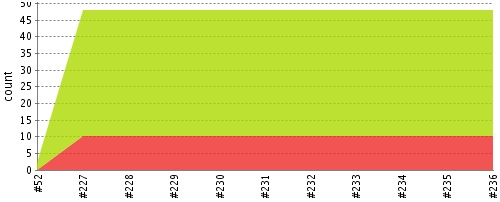
\includegraphics[width=0.5\textwidth]{test_graph}
  \label{fig:tests}
\end{figure}

\newpage

\section{Discussion}
\subsection{Architecture}
The architecture of AP2DX was well designed. What we thought off in the first week
was nearly exactly programmed when everything started to work (give or take a few
small details, which were easy to add). The framework is robust and more functionallity
can easily be added. For example; sensor messages we do not use can be added in mere moments 
by creating a specizialed message. 
\\\\
But, the question is: Is this a good thing? Obviously it is nice to see the framework working
and to know new functions can be added later. But it took us a loot of time to set it up. We 
did not need to parse all kind of special messages if only use two or three! 
\\\\
Also the base class disallowed us to test anything with the simulator until it was completely 
finished. Each module could easily be programmed in another programming language, but this
pinned us down to use Java, and the base class. 

\subsection{Message Protocols}
Parsing messages \\
We originally thought the messages for USAR and AP2DX were quite similar, but they diverged more
and more the further we came to working code. In the end it simply seemed as if we did the same
thing twice, with no real advantage. The USAR messages had to be parsed either way. They also
had to be compiled either way; there was no alternative method to communicate with the server. 
In hindsight, we might've better programmed that well, with a nice interface to set and get
variables rather than to program it twice. 


\newpage

\appendix
\appendixpage
\addappheadtotoc
\section{Constants}
In the sourcecode of the Planner there are some constants to tweak the behaviour of the robot, and there is one constant in the Reflex.

\subsection{Reflex}
\begin{itemize}
\item WALLDISTANCE: Sets the distance threshold for the mid six sonarsensors. If the sensor distance gets closer between two results, and the distance is less or equal to this constant, stop the robot. Given in meters. Default: 0.3
\end{itemize}

\subsection{Planner}
\begin{itemize}
\item ANGLEUNCERTAIN: threshold for turning to the ``angle'' direction, robot should drive in a direction between destinationAngle - ANGLEUNCERTAIN and destinationAngle + ANGLEUNCERTAIN. Given in radians. Default: 0.0872664626 (5 degrees)

\item TURNTHRESHOLD: This much should two sonardata results of one side sensor differ, before it will check the hole. In meters. Default: 1.0 

\item NEEDEDDEPTH: Mid four sonar sensors should be at least this deep to drive into hole. Given in meters. Default: 0.5

\item PASSHOLEDISTANCE: drive this much past a hole before restarting scan of environment. Given in meters. Default: 0.3

\item PASSHOLECORNER: drive this much past a hole before scanning it, so the bot is past the corner of the hole and not still partly infront of the wall. Given in meters. Default: 0.3

\item IGNOREDISTANCE: If distance from bot to wall (side sonar sensors) is larger than this, don't do hole checking. Because the bot is not following the wall. Given in meters. Default: 0.8

\item MOVEMENTTHRESHOLD: if movement is only this much between two INS data, then it is 'no movement'. Given in meters. Default: 0.2

\item NOMOVECOUNT: Did not move after this many INS data? Then action has to be taken. Default: 100

\item BACKWARDDISTANCE: If stuck, drive this much back. Given in meters. Default: 0.3

\end{itemize}
\section{UML Class diagram}
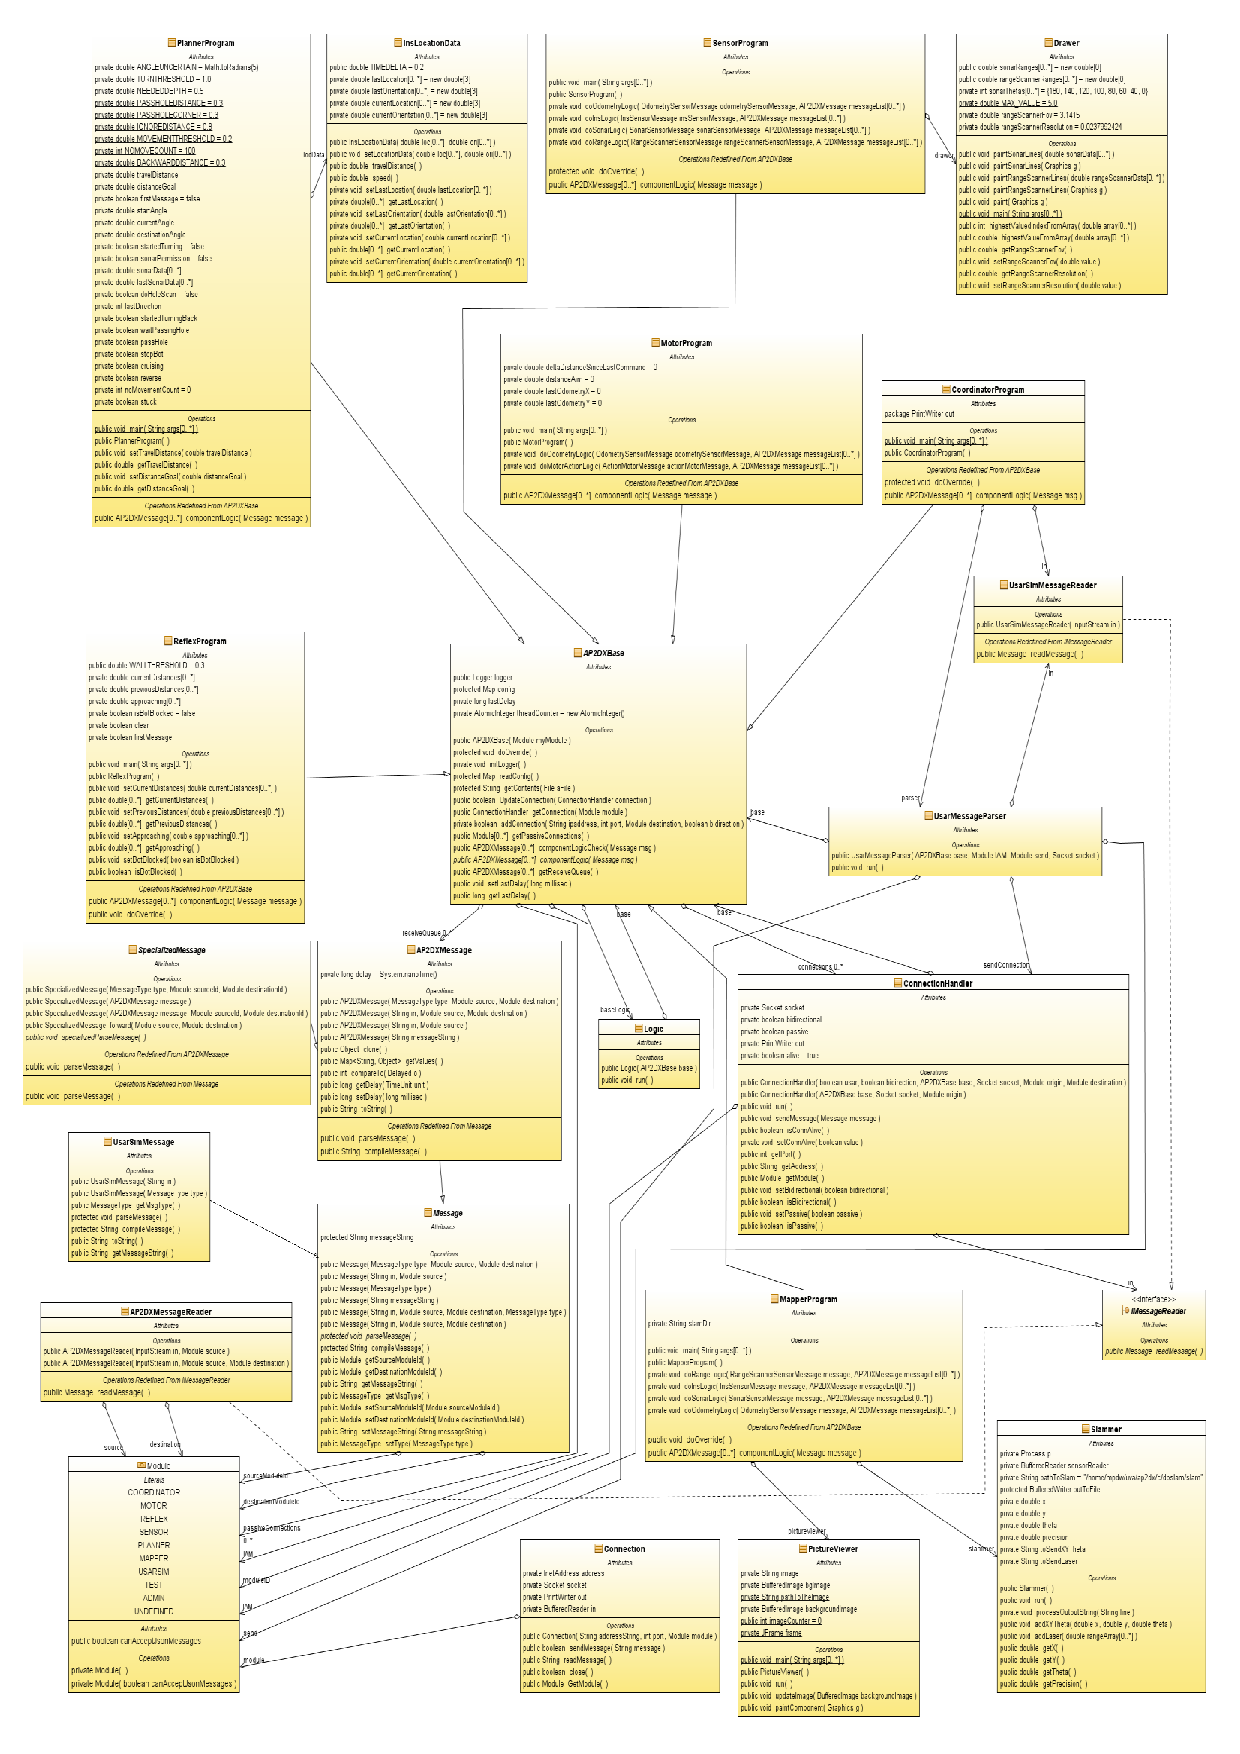
\includepdf{uml}
\end{document}

